\documentclass[11pt]{article}
\usepackage[margin=3cm, lmargin=2cm, rmargin=4cm, marginparwidth=3cm]{geometry}
\usepackage{graphicx, xcolor}
\usepackage{amsmath, amsfonts, amssymb, amsthm, mathtools, bm}
\usepackage{hyperref}
\usepackage[nameinlink]{cleveref}
\usepackage[all]{hypcap} % Links hyperref to object top and not caption
\usepackage[inline]{enumitem}
\usepackage{marginnote}

\title{Statistical and Mathematical Methods for Artificial Intelligence}
\date{2023 -- 2024}

\hypersetup{
    colorlinks,
    citecolor=black,
    filecolor=black,
    linkcolor=black,
    urlcolor=black,
    linktoc=all
}

\setlist[description]{labelindent=1em}   % Indents `description`
\setlength{\parindent}{0pt}
\renewcommand*{\marginfont}{\color{gray}\footnotesize}

\theoremstyle{definition}
\newtheorem{theorem}{Theorem}[section]
\newtheorem{example}{Example}[section]
\theoremstyle{definition}
\newtheorem*{definition}{Def}

\newcommand{\ubar}[1]{\text{\b{$#1$}}}
\renewcommand{\vec}[1]{{\bm{#1}}}
\newcommand{\nullvec}[0]{\bar{\vec{0}}}
\newcommand{\matr}[1]{{\bm{#1}}}


\begin{document}

    \makeatletter
    \begin{titlepage}
        \centering
        \vspace*{\fill}
        \huge
        \textbf{\@title}
        \vspace*{\fill}

        \Large
        Academic Year \@date\\
        Alma Mater Studiorum $\cdot$ University of Bologna
        \vspace*{1cm}
    \end{titlepage}
    \makeatother
    \pagenumbering{roman}
    \tableofcontents
    \newpage
    \pagenumbering{arabic}

    \chapter{Finite numbers}



\section{Sources of error}

\begin{description}
    \item[Measure error] \marginnote{Measure error}
        Precision of the measuring instrument.

    \item[Arithmetic error] \marginnote{Arithmetic error}
        Propagation of rounding errors in each step of an algorithm.

    \item[Truncation error] \marginnote{Truncation error}
        Approximating an infinite procedure to a finite number of iterations.

    \item[Inherent error] \marginnote{Inherent error}
        Caused by the finite representation of the data (floating-point).
        \begin{figure}[H]
            \centering
            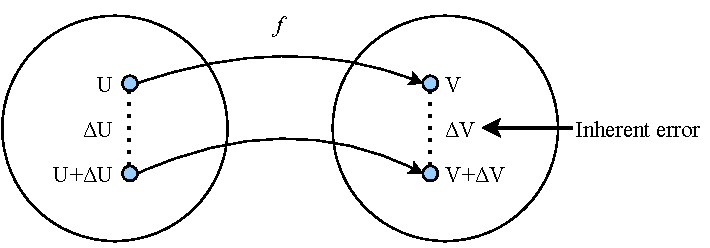
\includegraphics[width=0.6\textwidth]{img/_inherent_error.pdf}
            \caption{Inherent error visualization}
        \end{figure}
\end{description}



\section{Error measurement}

Let $x$ be a value and $\hat{x}$ its approximation. Then:
\begin{descriptionlist}
    \item[Absolute error] 
        \[
            E_{a} = \hat{x} - x 
            \marginnote{Absolute error}
        \] 
        Note that, out of context, the absolute error is meaningless.
    \item[Relative error] 
        \[
            E_{r} = \frac{\hat{x} - x}{x} 
            \marginnote{Relative error}
        \] 
\end{descriptionlist}



\section{Representation in base \texorpdfstring{$\beta$}{B}}

Let $\beta \in \mathbb{N}_{> 1}$ be the base.
Each $x \in \mathbb{R} \smallsetminus \{0\}$ can be uniquely represented as:
\begin{equation}
    \label{eq:finnum_b_representation}
    x = \texttt{sign}(x) \cdot (d_1\beta^{-1} + d_2\beta^{-2} + \dots + d_n\beta^{-n})\beta^p
\end{equation}
where:
\begin{itemize}
    \item $0 \leq d_i \leq \beta-1$
    \item $d_1 \neq 0$
    \item starting from an index $i$, not all $d_j$ ($j \geq i$) are equal to $\beta-1$
\end{itemize}
%
\Cref{eq:finnum_b_representation} can be represented using the normalized scientific notation as: \marginnote{Normalized scientific notation}
\[
    x = \pm (0.d_1d_2\dots) \beta^p
\]
where $0.d_1d_2\dots$ is the \textbf{mantissa} and $\beta^p$ the \textbf{exponent}. \marginnote{Mantissa\\Exponent}



\section{Floating-point}
A floating-point system $\mathcal{F}(\beta, t, L, U)$ is defined by the parameters: \marginnote{Floating-point}
\begin{itemize}
    \item $\beta$: base
    \item $t$: precision (number of digits in the mantissa)
    \item $[L, U]$: range of the exponent
\end{itemize}

Each $x \in \mathcal{F}(\beta, t, L, U)$ can be represented in its normalized form:
\begin{eqnarray}
    x = \pm (0.d_1d_2 \dots d_t) \beta^p & L \leq p \leq U
\end{eqnarray}
We denote with $\texttt{fl}(x)$ the representation of $x \in \mathbb{R}$ in a given floating-point system.

\begin{example}
    In $\mathcal{F}(10, 5, -3, 3)$, $x=12.\bar{3}$ is represented as:
    \begin{equation*}
        \texttt{fl}(x) = + 0.12333 \cdot 10^2
    \end{equation*}
\end{example}


\subsection{Numbers distribution}
Given a floating-point system $\mathcal{F}(\beta, t, L, U)$, the total amount of representable numbers is:
\begin{equation*}
    2(\beta-1) \beta^{t-1} (U-L+1)+1
\end{equation*}
%
Representable numbers are more sparse towards the exponent upper bound and more dense towards the lower bound.
It must be noted that there is an underflow area around 0.
\begin{figure}[H]
    \centering
    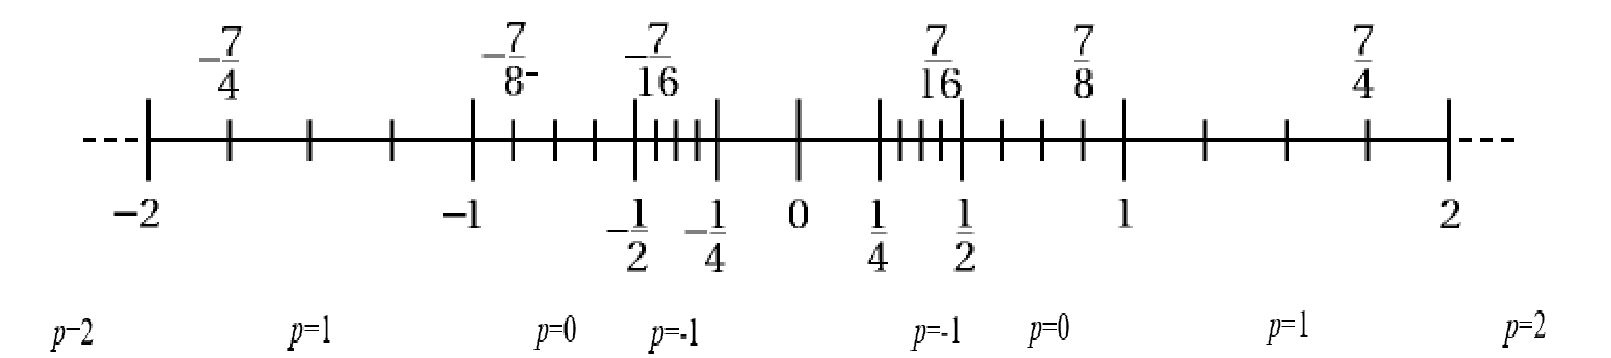
\includegraphics[width=0.8\textwidth]{img/floatingpoint_range.png}
    \caption{Floating-point numbers in $\mathcal{F}(2, 3, -1, 2)$}
\end{figure}


\subsection{Number representation}
Given a floating-point system $\mathcal{F}(\beta, t, L, U)$, the representation of $x \in \mathbb{R}$ can result in:
\begin{descriptionlist}
    \item[Exact representation] 
        if $p \in [L, U]$ and $d_i=0$ for $i>t$.

    \item[Approximation] \marginnote{Truncation\\Rounding}
        if $p \in [L, U]$ but $d_i$ may not be 0 for $i>t$. 
        In this case, the representation is obtained by truncating or rounding the value.

    \item[Underflow] \marginnote{Underflow}
        if $p < L$. In this case, the value is approximated to 0.

    \item[Overflow] \marginnote{Overflow}
        if $p > U$. In this case, an exception is usually raised.
\end{descriptionlist}


\subsection{Machine precision}
Machine precision $\varepsilon_{\text{mach}}$ determines the accuracy of a floating-point system. \marginnote{Machine precision}
Depending on the approximation approach, machine precision can be computed as:
\begin{descriptionlist}
    \item[Truncation] $\varepsilon_{\text{mach}} = \beta^{1-t}$
    \item[Rounding] $\varepsilon_{\text{mach}} = \frac{1}{2}\beta^{1-t}$
\end{descriptionlist}
Therefore, rounding results in more accurate representations.

$\varepsilon_{\text{mach}}$ is the smallest distance among the representable numbers (\Cref{fig:finnum_eps}).
\begin{figure}[H]
    \centering
    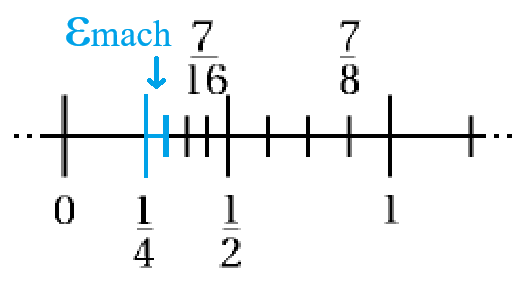
\includegraphics[width=0.2\textwidth]{img/machine_eps.png}
    \caption{Visualization of $\varepsilon_{\text{mach}}$ in $\mathcal{F}(2, 3, -1, 2)$}
    \label{fig:finnum_eps}
\end{figure}

In alternative, $\varepsilon_{\text{mach}}$ can be defined as the smallest representable number such that:
\begin{equation*}
    \texttt{fl}(1 + \varepsilon_{\text{mach}}) > 1.
\end{equation*}


\subsection{IEEE standard}
IEEE 754 defines two floating-point formats:
\begin{descriptionlist}
    \item[Single precision] Stored in 32 bits. Represents the system $\mathcal{F}(2, 24, -128, 127)$. \marginnote{\texttt{float32}}
        \begin{center}
            \small
            \begin{tabular}{|c|c|c|}
                \hline
                1 (sign) & 8 (exponent) & 23 (mantissa) \\
                \hline
            \end{tabular}
        \end{center}

    \item[Double precision] Stored in 64 bits. Represents the system $\mathcal{F}(2, 53, -1024, 1023)$. \marginnote{\texttt{float64}}
        \begin{center}
            \small
            \begin{tabular}{|c|c|c|}
                \hline
                1 (sign) & 11 (exponent) & 52 (mantissa) \\
                \hline
            \end{tabular}
        \end{center}
\end{descriptionlist}
As the first digit of the mantissa is always 1, it does not need to be stored.
Moreover, special configurations are reserved to represent \texttt{Inf} and \texttt{NaN}.


\subsection{Floating-point arithmetic}
Let:
\begin{itemize}
    \item $+: \mathbb{R} \times \mathbb{R} \rightarrow \mathbb{R}$ be a real numbers operation.
    \item $\oplus: \mathcal{F} \times \mathcal{F} \rightarrow \mathcal{F}$ be the corresponding operation in a floating-point system.
\end{itemize}
%
To compute $x \oplus y$, a machine:
\begin{enumerate}
    \item Calculates $x + y$ in a high precision register 
        (still approximated, but more precise than the floating-point system used to store the result)
    \item Stores the result as $\texttt{fl}(x + y)$
\end{enumerate}

A floating-point operation causes a small rounding error:
\[
    \left\vert \frac{(x \oplus y) - (x + y)}{x+y} \right\vert < \varepsilon_{\text{mach}}
\]
%
However, some operations may be subject to the \textbf{cancellation} problem which causes information loss.
\marginnote{Cancellation}
\begin{example}
    Given $x = 1$ and $y = 1 \cdot 10^{-17}$, we want to compute $x + y$ in $\mathcal{F}(10, 16, U, L)$.
    It is assumed that $U$ and $L$ are sufficient for this example.
    \begin{equation*}
        \begin{split}
            z & = \texttt{fl}(x) + \texttt{fl}(y) \\
              & = 0.1 \cdot 10^1 + 0.1 \cdot 10^{-16} \\
              & = (0.1 + 0.\overbrace{0\dots0}^{\mathclap{16\text{ zeros}}}1) \cdot 10^1 \\
              & = 0.1\overbrace{0\dots0}^{\mathclap{15\text{ zeros}}}1 \cdot 10^1
        \end{split}
    \end{equation*}
    Then, we have that $\texttt{fl}(z) = 0.1\overbrace{0\dots0}^{\mathclap{15\text{ zeros}}} \cdot 10^1 = 1 = x$.
\end{example}
    \newpage
    \chapter{Linear algebra}


\section{Vector space}

A \textbf{vector space} over $\mathbb{R}$ is a nonempty set $V$, whose elements are called vectors, with two operations: 
\marginnote{Vector space}
\begin{center}
    \begin{tabular}{l c}
        Addition & $+ : V \times V \rightarrow V$ \\
        Scalar multiplication & $\cdot : \mathbb{R} \times V \rightarrow V$
    \end{tabular}
\end{center}
A vector space has the following properties:
\begin{enumerate}
    \item Addition is commutative and associative
    \item A null vector exists: $\exists \nullvec \in V$ s.t. $\forall \vec{u} \in V: \nullvec + \vec{u} = \vec{u} + \nullvec = \vec{u}$
    \item An identity element for scalar multiplication exists: $\forall \vec{u} \in V: 1\vec{u} = \vec{u}$
    \item Each vector has its opposite: $\forall \vec{u} \in V, \exists \vec{a} \in V: \vec{a} + \vec{u} = \vec{u} + \vec{a} = \nullvec$.\\
        $\vec{a}$ is denoted as $-\vec{u}$.
    \item Distributive properties:
        \[ \forall \alpha \in \mathbb{R}, \forall \vec{u}, \vec{w} \in V: \alpha(\vec{u} + \vec{w}) = \alpha \vec{u} + \alpha \vec{w} \]
        \[ \forall \alpha, \beta \in \mathbb{R}, \forall \vec{u} \in V: (\alpha + \beta)\vec{u} = \alpha \vec{u} + \beta \vec{u} \]
    \item Associative property:
        \[ \forall \alpha, \beta \in \mathbb{R}, \forall \vec{u} \in V: (\alpha \beta)\vec{u} = \alpha (\beta \vec{u}) \]
\end{enumerate}
%
A subset $U \subseteq V$ of a vector space $V$ is a \textbf{subspace} iff $U$ is a vector space.
\marginnote{Subspace}


\subsection{Basis}
\marginnote{Basis}
Let $V$ be a vector space of dimension $n$.
A basis $\beta = \{ \vec{v}_1, \dots, \vec{v}_n \}$ of $V$ is a set of $n$ linearly independent vectors of $V$.\\ 
Each element of $V$ can be represented as a linear combination of the vectors in the basis $\beta$:
\[ \forall \vec{w} \in V: \vec{w} = \lambda_1\vec{v}_1 + \dots + \lambda_n\vec{v}_n \text{ where } \lambda_i \in \mathbb{R} \]
%
The canonical basis of a vector space is a basis where each vector represents a dimension $i$ \marginnote{Canonical basis}
(i.e. 1 in position $i$ and 0 in all other positions).
\begin{example}
    The canonical basis $\beta$ of $\mathbb{R}^3$ is $\beta = \{ (1, 0, 0), (0, 1, 0), (0, 0, 1) \}$
\end{example}

\subsection{Dot product}
The dot product of two vectors in $\vec{x}, \vec{y} \in \mathbb{R}^n$ is defined as: \marginnote{Dot product}
\begin{equation*}
    \left\langle \vec{x}, \vec{y} \right\rangle =
    \vec{x}^T \vec{y} = \sum_{i=1}^{n} x_i \cdot y_i
\end{equation*}


\section{Matrix}

This is a {\tiny(very formal definition of)} matrix: \marginnote{Matrix}
\begin{equation*}
    \matr{A} =
    \begin{pmatrix}
        a_{11} & a_{12} & \dots  & a_{1n} \\
        a_{21} & a_{22} & \dots  & a_{2n} \\
        \vdots & \vdots & \ddots & \vdots \\
        a_{m1} & a_{m2} & \dots  & a_{mn}
    \end{pmatrix}
\end{equation*}

\subsection{Invertible matrix}
A matrix $\matr{A} \in \mathbb{R}^{n \times n}$ is invertible (non-singular) if: \marginnote{Non-singular matrix}
\begin{equation*}
    \exists \matr{B} \in \mathbb{R}^{n \times n}: \matr{AB} = \matr{BA} = \matr{I}
\end{equation*}
where $\matr{I}$ is the identity matrix. $\matr{B}$ is denoted as $\matr{A}^{-1}$.

\subsection{Kernel}
The null space (kernel) of a matrix $\matr{A} \in \mathbb{R}^{m \times n}$ is a subspace such that: \marginnote{Kernel}
\begin{equation*}
    \text{Ker}(\matr{A}) = \{ \vec{x} \in \mathbb{R}^n : \matr{A}\vec{x} = \nullvec \}
\end{equation*}
%
\begin{theorem} \label{th:kernel_invertible}
    A square matrix $\matr{A}$ with $\text{\normalfont Ker}(\matr{A}) = \{\nullvec\}$ is non singular.
\end{theorem}

\subsection{Similar matrices} \marginnote{Similar matrices}
Two matrices $\matr{A}$ and $\matr{D}$ are \textbf{similar} if there exists an invertible matrix $\matr{P}$ such that:
\[ \matr{D} = \matr{P}^{-1} \matr{A} \matr{P} \]



\section{Norms}

\subsection{Vector norms}
The norm of a vector is a function: \marginnote{Vector norm}
\begin{equation*}
    \Vert \cdot \Vert: \mathbb{R}^n \rightarrow \mathbb{R}
\end{equation*}
such that for each $\lambda \in \mathbb{R}$ and $\vec{x}, \vec{y} \in \mathbb{R}^n$:
\begin{itemize}
    \item $\Vert \vec{x} \Vert \geq 0$
    \item $\Vert \vec{x} \Vert = 0 \iff \vec{x} = \nullvec$
    \item $\Vert \lambda \vec{x} \Vert = \vert \lambda \vert \cdot \Vert \vec{x} \Vert$
    \item $\Vert \vec{x} + \vec{y} \Vert \leq \Vert \vec{x} \Vert + \Vert \vec{y} \Vert$
\end{itemize}
%
Common norms are:
\begin{descriptionlist}
    \item[2-norm] $\Vert \vec{x} \Vert_2 = \sqrt{ \sum_{i=1}^{n} x_i^2 }$
    
    \item[1-norm] $\Vert \vec{x} \Vert_1 = \sum_{i=1}^{n} \vert x_i \vert$
    
    \item[$\infty$-norm] $\Vert \vec{x} \Vert_{\infty} = \max_{1 \leq i \leq n} \vert x_i \vert$
\end{descriptionlist}
%
In general, different norms tend to maintain the same proportion.
In some cases, unbalanced results may be obtained when comparing different norms.
\begin{example}
    Let $\vec{x} = (1, 1000)$ and $\vec{y} = (999, 1000)$. Their norms are:
    \begin{center}
        \begin{tabular}{l l}
            $\Vert \vec{x} \Vert_{2} = \sqrt{1000001}$ & $\Vert \vec{y} \Vert_{2} = \sqrt{1998001}$ \\
            $\Vert \vec{x} \Vert_{\infty} = 1000$ & $\Vert \vec{y} \Vert_{\infty} = 1000$ \\
        \end{tabular} 
    \end{center}
\end{example}


\subsection{Matrix norms}
The norm of a matrix is a function: \marginnote{Matrix norm}
\begin{equation*}
    \Vert \cdot \Vert: \mathbb{R}^{m \times n} \rightarrow \mathbb{R}
\end{equation*}
such that for each $\lambda \in \mathbb{R}$ and $\matr{A}, \matr{B} \in \mathbb{R}^{m \times n}$:
\begin{itemize}
    \item $\Vert \matr{A} \Vert \geq 0$
    \item $\Vert \matr{A} \Vert = 0 \iff \matr{A} = \matr{0}$
    \item $\Vert \lambda \matr{A} \Vert = \vert \lambda \vert \cdot \Vert \matr{A} \Vert$
    \item $\Vert \matr{A} + \matr{B} \Vert \leq \Vert \matr{A} \Vert + \Vert \matr{B} \Vert$
\end{itemize}
%
Common norms are:
\begin{descriptionlist}
    \item[2-norm] 
        $\Vert \matr{A} \Vert_2 = \sqrt{ \rho(\matr{A}^T\matr{A}) }$,\\
        where $\rho(\matr{X})$ is the largest absolute value of the eigenvalues of $\matr{X}$ (spectral radius).
    
    \item[1-norm] $\Vert \matr{A} \Vert_1 = \max_{1 \leq j \leq n} \sum_{i=1}^{m} \vert a_{i,j} \vert$ (i.e. max sum of the columns in absolute value)
    
    \item[Frobenius norm] $\Vert \matr{A} \Vert_F = \sqrt{ \sum_{i=1}^{m} \sum_{j=1}^{n} a_{i,j}^2 }$
\end{descriptionlist}



\section{Symmetric, positive definite matrices}

\begin{description}
    \item[Symmetric matrix] \marginnote{Symmetric matrix}
        A square matrix $\matr{A} \in \mathbb{R}^{n \times n}$ is symmetric $\iff \matr{A} = \matr{A}^T$
    
    \item[Positive semidefinite matrix] \marginnote{Positive semidefinite matrix}
        A symmetric matrix $\matr{A} \in \mathbb{R}^{n \times n}$ is positive semidefinite iff
        \begin{equation*}
            \forall \vec{x} \in \mathbb{R}^n \smallsetminus \{0\}: \vec{x}^T \matr{A} \vec{x} \geq 0
        \end{equation*}

    \item[Positive definite matrix] \marginnote{Positive definite matrix}
        A symmetric matrix $\matr{A} \in \mathbb{R}^{n \times n}$ is positive definite iff
        \begin{equation*}
            \forall \vec{x} \in \mathbb{R}^n \smallsetminus \{0\}: \vec{x}^T \matr{A} \vec{x} > 0
        \end{equation*}
        %
        It has the following properties:
        \begin{enumerate}
            \item The null space of $\matr{A}$ has the null vector only: $\text{Ker}(\matr{A}) = \{ \nullvec \}$. \\
                Which implies that $\matr{A}$ is non-singular (\Cref{th:kernel_invertible}).
            \item The diagonal elements of $\matr{A}$ are all positive.
        \end{enumerate}
\end{description}



\section{Orthogonality}
\begin{description}
    \item[Angle between vectors] \marginnote{Angle between vectors}
        The angle $\omega$ between two vectors $\vec{x}$ and $\vec{y}$ can be obtained from:
        \begin{equation*}
            \cos\omega = \frac{\left\langle \vec{x}, \vec{y} \right\rangle }{\Vert \vec{x} \Vert_2 \cdot \Vert \vec{y} \Vert_2}
        \end{equation*}
    
    \item[Orthogonal vectors] \marginnote{Orthogonal vectors}
        Two vectors $\vec{x}$ and $\vec{y}$ are orthogonal ($\vec{x} \perp \vec{y}$) when:
        \[ \left\langle \vec{x}, \vec{y} \right\rangle = 0 \]
    
    \item[Orthonormal vectors] \marginnote{Orthonormal vectors}
        Two vectors $\vec{x}$ and $\vec{y}$ are orthonormal when:
        \[ \vec{x} \perp \vec{y} \text{ and } \Vert \vec{x} \Vert = \Vert \vec{y} \Vert=1 \]
        \begin{theorem}
            The canonical basis of a vector space is orthonormal.
        \end{theorem}
    
    \item[Orthogonal matrix] \marginnote{Orthogonal matrix}
        A matrix $\matr{A} \in \mathbb{R}^{n \times n}$ is orthogonal if its columns are \underline{orthonormal} vectors.
        It has the following properties:
        \begin{enumerate}
            \item $\matr{A}\matr{A}^T = \matr{I} = \matr{A}^T\matr{A}$, which implies $\matr{A}^{-1} = \matr{A}^T$.
            \item The length of a vector is unchanged when mapped through an orthogonal matrix: 
                \[ \Vert \matr{A}\vec{x} \Vert^2 = \Vert \vec{x} \Vert^2 \]
            \item The angle between two vectors is unchanged when both are mapped through an orthogonal matrix:
                \[ 
                    \cos\omega = \frac{(\matr{A}\vec{x})^T(\matr{A}\vec{y})}{\Vert \matr{A}\vec{x} \Vert \cdot \Vert \matr{A}\vec{y} \Vert} = 
                        \frac{\vec{x}^T\vec{y}}{\Vert \vec{x} \Vert \cdot \Vert \vec{y} \Vert}
                \]
        \end{enumerate}
        Note: an orthogonal matrix represents a rotation.

    \item[Orthogonal basis] \marginnote{Orthogonal basis}
        Given a $n$-dimensional vector space $V$ and a basis $\beta = \{ \vec{b}_1, \dots, \vec{b}_n \}$ of $V$.
        $\beta$ is an orthogonal basis if:
        \[ \vec{b}_i \perp \vec{b}_j \text{ for } i \neq j \text{ (i.e.} \left\langle \vec{b}_i, \vec{b}_j \right\rangle = 0 \text{)} \]

    \item[Orthonormal basis] \marginnote{Orthonormal basis}
        Given a $n$-dimensional vector space $V$ and an orthogonal basis $\beta = \{ \vec{b}_1, \dots, \vec{b}_n \}$ of $V$.
        $\beta$ is an orthonormal basis if:
        \[ \Vert \vec{b}_i \Vert_2 = 1 \text{ (or} \left\langle \vec{b}_i, \vec{b}_i \right\rangle = 1 \text{)} \]
    
    \item[Orthogonal complement] \marginnote{Orthogonal complement}
        Given a $n$-dimensional vector space $V$ and a $m$-dimensional subspace $U \subseteq V$.
        The orthogonal complement $U^\perp$ of $U$ is a $(n-m)$-dimensional subspace of $V$ such that it
        contains all the vectors orthogonal to every vector in $U$:
        \[ \forall \vec{w} \in V: \vec{w} \in U^\perp \iff (\forall \vec{u} \in U: \vec{w} \perp \vec{u}) \]
        %
        Note that $U \cap U^\perp = \{ \nullvec \}$ and 
        it is possible to represent all vectors in $V$ as a linear combination of both the basis of $U$ and $U^\perp$.
        
        The vector $\vec{w} \in U^\perp$ s.t. $\Vert \vec{w} \Vert = 1$ is the \textbf{normal vector} of $U$. \marginnote{Normal vector}
        %
        \begin{figure}[h]
            \centering
            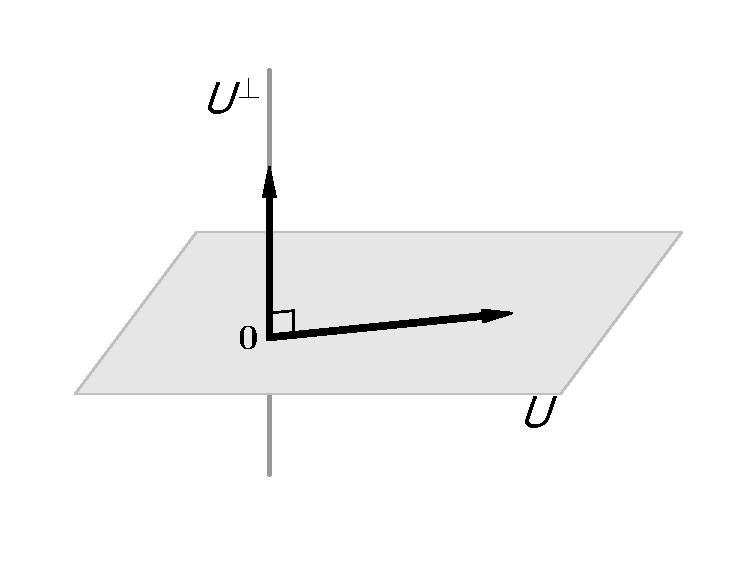
\includegraphics[width=0.4\textwidth]{img/_orthogonal_complement.pdf}
            \caption{Orthogonal complement of a subspace $U \subseteq \mathbb{R}^3$}
        \end{figure}
\end{description}



\section{Projections}
Projections are methods to map high-dimensional data into a lower-dimensional space 
while minimizing the compression loss.\\
\marginnote{Orthogonal projection}
Let $V$ be a vector space and $U \subseteq V$ a subspace of $V$.
A linear mapping $\pi: V \rightarrow U$ is a (orthogonal) projection if:
\[ \pi^2 = \pi \circ \pi = \pi \]
In other words, applying $\pi$ multiple times gives the same result (i.e. idempotency).\\
$\pi$ can be expressed as a transformation matrix $\matr{P}_\pi$ such that:
\[ \matr{P}_\pi^2 = \matr{P}_\pi \] 

\subsection{Projection onto general subspaces} \marginnote{Projection onto subspace basis}
To project a vector $\vec{x} \in \mathbb{R}^n$ into a lower-dimensional subspace $U \subseteq \mathbb{R}^n$,
it is possible to use the basis of $U$.\\
%
Let $m = \text{dim}(U)$ be the dimension of $U$ and 
$\matr{B} = (\vec{b}_1, \dots, \vec{b}_m) \in \mathbb{R}^{n \times m}$ an ordered basis of $U$.
A projection $\pi_U(\vec{x})$ represents $\vec{x}$ as a linear combination of the basis:
\[ \pi_U(\vec{x}) = \sum_{i=1}^{m} \lambda_i \vec{b}_i = \matr{B}\vec{\lambda} \]
where $\vec{\lambda} = (\lambda_1, \dots, \lambda_m)^T \in \mathbb{R}^{m}$ are the new coordinates of $\vec{x}$ 
and is found by minimizing the distance between $\pi_U(\vec{x})$ and $\vec{x}$.



\section{Eigenvectors and eigenvalues}

Given a square matrix $\matr{A} \in \mathbb{R}^{n \times n}$, 
$\lambda \in \mathbb{C}$ is an eigenvalue of $\matr{A}$ \marginnote{Eigenvalue}
with corresponding eigenvector $\vec{x} \in \mathbb{R}^n \smallsetminus \{ \nullvec \}$ if: \marginnote{Eigenvector}
\[ \matr{A}\vec{x} = \lambda\vec{x} \]

It is equivalent to say that:
\begin{itemize}
    \item $\lambda$ is an eigenvalue of $\matr{A} \in \mathbb{R}^{n \times n}$
    \item $\exists \vec{x} \in \mathbb{R}^n \smallsetminus \{ \nullvec \}$ s.t. $\matr{A}\vec{x} = \lambda\vec{x}$ \\
        Equivalently the system $(\matr{A} - \lambda \matr{I}_n)\vec{x} = \nullvec$ is non-trivial ($\vec{x} \neq \nullvec$).
    \item $\text{rank}(\matr{A} - \lambda \matr{I}_n) < n$
    \item $\det(\matr{A} - \lambda \matr{I}_n) = 0$ (i.e. $(\matr{A} - \lambda \matr{I}_n)$ is singular {\footnotesize(i.e. not invertible)})
\end{itemize}

Note that eigenvectors are not unique.
Given an eigenvector $\vec{x}$ of $\matr{A}$ with eigenvalue $\lambda$, 
we can prove that $\forall c \in \mathbb{R} \smallsetminus \{0\}:$ $c\vec{x}$ is an eigenvector of $\matr{A}$:
\[ \matr{A}(c\vec{x}) = c(\matr{A}\vec{x}) = c\lambda\vec{x} = \lambda(c\vec{x}) \]

% \begin{theorem}
%     The eigenvalues of a symmetric matrix $\matr{A} \in \mathbb{R}^{n \times n}$ are all in $\mathbb{R}$.
% \end{theorem}

\begin{theorem} \marginnote{Eigenvalues and positive definiteness}
    $\matr{A} \in \mathbb{R}^{n \times n}$ is symmetric positive definite $\iff$
    its eigenvalues are all positive.
\end{theorem}

\begin{description}
    \item[Eigenspace] \marginnote{Eigenspace}
        Set of all the eigenvectors of $\matr{A} \in \mathbb{R}^{n \times n}$ associated to an eigenvalue $\lambda$.
        This set is a subspace of $\mathbb{R}^n$.
    
    \item[Eigenspectrum] \marginnote{Eigenspectrum}
        Set of all eigenvalues of $\matr{A} \in \mathbb{R}^{n \times n}$.
\end{description}


\begin{description}
    \item[Geometric multiplicity] \marginnote{Geometric multiplicity}
        Given an eigenvalue $\lambda$ of a matrix $\matr{A} \in \mathbb{R}^{n \times n}$.
        The geometric multiplicity of $\lambda$ is the number of linearly independent eigenvectors associated to $\lambda$.
\end{description}


\begin{theorem} \marginnote{Linearly independent eigenvectors}
    Given a matrix $\matr{A} \in \mathbb{R}^{n \times n}$. 
    If its $n$ eigenvectors $\vec{x}_1, \dots, \vec{x}_n$ are associated to distinct eigenvalues, 
    then $\vec{x}_1, \dots, \vec{x}_n$ are linearly independent (i.e. they form a basis of $\mathbb{R}^n$).

    \begin{descriptionlist}
        \item[Defective matrix] \marginnote{Defective matrix}
            A matrix $\matr{A} \in \mathbb{R}^{n \times n}$ is defective if it has less than $n$ linearly independent eigenvectors.
    \end{descriptionlist}
\end{theorem}


\begin{theorem}[Spectral theorem] \marginnote{Spectral theorem}
    Given a symmetric matrix $\matr{A} \in \mathbb{R}^{n \times n}$.
    Its eigenvectors form a orthonormal basis and its eigenvalues are all in $\mathbb{R}$.
\end{theorem}


\subsection{Diagonalizability}
\marginnote{Diagonalizable matrix}
A matrix $\matr{A} \in \mathbb{R}^{n \times n}$ is diagonalizable if it is similar to a diagonal matrix $\matr{D} \in \mathbb{R}^{n \times n}$:
\[ \exists \matr{P} \in \mathbb{R}^{n \times n} \text{ s.t. } \matr{P} \text{ invertible and } \matr{D} = \matr{P}^{-1}\matr{A}\matr{P} \]

\begin{theorem}
    Similar matrices have the same eigenvalues.
\end{theorem}

\begin{theorem} \marginnote{Symmetric matrix diagonalizability}
    A symmetric matrix $\matr{A} \in \mathbb{R}^{n \times n}$ is always diagonalizable.
\end{theorem}
    \newpage
    \chapter{Linear systems}

A linear system:
\begin{equation*}
    \begin{cases}
        a_{1,1}x_1 + a_{1,2}x_2 + \dots + a_{1,n}x_n = b_1\\
        a_{2,1}x_1 + a_{2,2}x_2 + \dots + a_{2,n}x_n = b_2\\
        \hspace*{7em} \vdots \\
        a_{m,1}x_1 + a_{m,2}x_2 + \dots + a_{m,n}x_n = b_m\\
    \end{cases}
\end{equation*}
can be represented as:
\[ \matr{A}\vec{x} = \vec{b} \]
where:
\[
    \matr{A} = 
    \begin{pmatrix}
        a_{1,1} & a_{1, 2} & \hdots & a_{1,n} \\
        a_{2,1} & a_{2, 2} & \hdots & a_{2,n} \\
        \vdots  & \vdots   & \ddots & \vdots  \\
        a_{m,1} & a_{m, 2} & \hdots & a_{m,n}
    \end{pmatrix} \in \mathbb{R}^{m \times n}
    \hspace*{2em}
    %
    \vec{x} = 
    \begin{pmatrix}
        x_1 \\
        x_2 \\ 
        \vdots \\
        x_n
    \end{pmatrix} \in \mathbb{R}^n
    \hspace*{2em}
    %
    \vec{b} = 
    \begin{pmatrix}
        b_1 \\
        b_2 \\ 
        \vdots \\
        b_m
    \end{pmatrix} \in \mathbb{R}^m
\]
    


\section{Square linear systems}
\marginnote{Square linear system}
A square linear system $\matr{A}\vec{x} = \vec{b}$ with $\matr{A} \in \mathbb{R}^{n \times n}$ and $\vec{x}, \vec{b} \in \mathbb{R}^n$
has an unique solution iff one of the following conditions is satisfied:
\begin{enumerate}
    \item $\matr{A}$ is non-singular (invertible)
    \item $\text{rank}(\matr{A}) = n$ (full rank)
    \item $\matr{A}\vec{x}$ admits only the solution $\vec{x} = \nullvec$
\end{enumerate}

The solution can be algebraically determined as \marginnote{Algebraic solution to linear systems}
\[ \matr{A}\vec{x} = \vec{b} \iff \vec{x} = \matr{A}^{-1}\vec{b} \]
However this approach requires to compute the inverse of a matrix, which has a time complexity of $O(n^3)$.



\section{Direct methods}
\marginnote{Direct methods}
Direct methods compute the solution of a linear system in a finite number of steps.
Compared to iterative methods, they are more precise but more expensive.

The most common approach consists in factorizing the matrix $\matr{A}$.

\subsection{Gaussian factorization}
\marginnote{Gaussian factorization\\(LU decomposition)}
Given a square linear system $\matr{A}\vec{x} = \vec{b}$, 
the matrix $\matr{A} \in \mathbb{R}^{n \times n}$ is factorized into $\matr{A} = \matr{L}\matr{U}$ such that:
\begin{itemize}
    \item $\matr{L} \in \mathbb{R}^{n \times n}$ is a lower triangular matrix
    \item $\matr{U} \in \mathbb{R}^{n \times n}$ is an upper triangular matrix
\end{itemize}
%
As directly solving a system with a triangular matrix has complexity $O(n^2)$ (forward or backward substitutions), 
the system can be decomposed to:
\begin{equation}
    \begin{split}
        \matr{A}\vec{x} = \vec{b} & \iff \matr{LU}\vec{x} = \vec{b} \\
            & \iff \vec{y} = \matr{U}\vec{x} \text{ \& } \matr{L}\vec{y} = \vec{b}
    \end{split}
\end{equation}
To find the solution, it is sufficient to solve in order:
\begin{enumerate}
    \item $\matr{L}\vec{y} = \vec{b}$ (solved w.r.t. $\vec{y}$)
    \item $\vec{y} = \matr{U}\vec{x}$ (solved w.r.t. $\vec{x}$)
\end{enumerate}

The overall complexity is $O(\frac{n^3}{3}) + 2 \cdot O(n^2) = O(\frac{n^3}{3})$

\subsection{Gaussian factorization with pivoting}
\marginnote{Gaussian factorization with pivoting}
During the computation of $\matr{A} = \matr{L}\matr{U}$ 
(using Gaussian elimination\footnote{\url{https://en.wikipedia.org/wiki/LU\_decomposition\#Using\_Gaussian\_elimination}}), 
a division by 0 may occur.
A method to prevent this problem (and to lower the algorithmic error) is to change the order of the rows of $\matr{A}$ before decomposing it.
This is achieved by using a permutation matrix $\matr{P}$, which is obtained as a permutation of the identity matrix.

The permuted system becomes $\matr{P}\matr{A}\vec{x} = \matr{P}\vec{b}$ and the factorization is obtained as $\matr{P}\matr{A} = \matr{L}\matr{U}$.
The system can be decomposed to:
\begin{equation}
    \begin{split}
        \matr{P}\matr{A}\vec{x} = \matr{P}\vec{b} & \iff \matr{L}\matr{U}\vec{x} = \matr{P}\vec{b} \\
            & \iff \vec{y} = \matr{U}\vec{x} \text{ \& } \matr{L}\vec{y} = \matr{P}\vec{b}
    \end{split}
\end{equation}

An alternative formulation (which is what \texttt{SciPy} uses) 
is defined as:
\[\matr{A} = \matr{P}\matr{L}\matr{U} \iff \matr{P}^T\matr{A} = \matr{L}\matr{U} \]
It must be noted that $\matr{P}$ is orthogonal, so $\matr{P}^T = \matr{P}^{-1}$.
The solution to the system ($\matr{P}^T\matr{A}\vec{x} = \matr{P}^T\vec{b}$) can be found as above.



\section{Iterative methods}
\marginnote{Iterative methods}
Iterative methods solve a linear system by computing a sequence that converges to the exact solution.
Compared to direct methods, they are less precise but computationally faster and more adapt for large systems. 

The overall idea is to build a sequence of vectors $\vec{x}_k$ 
that converges to the exact solution $\vec{x}^*$:
\[ \lim_{k \rightarrow \infty} \vec{x}_k = \vec{x}^* \]
Generally, the first vector $\vec{x}_0$ is given (or guessed). Subsequent vectors are computed w.r.t. the previous iteration 
as $\vec{x}_k = g(\vec{x}_{k-1})$.

The two most common families of iterative methods are:
\begin{descriptionlist}
    \item[Stationary methods] \marginnote{Stationary methods}
        compute the sequence as:
        \[ \vec{x}_k = \matr{B}\vec{x}_{k-1} + \vec{d} \]
        where $\matr{B}$ is called iteration matrix and $\vec{d}$ is computed from the $\vec{b}$ vector of the system.
        The time complexity per iteration $O(n^2)$.
    
    \item[Gradient-like methods] \marginnote{Gradient-like methods}
        have the form:
        \[ \vec{x}_k = \vec{x}_{k-1} + \alpha_{k-1}\vec{p}_{k-1} \]
        where $\alpha_{k-1} \in \mathbb{R}$ and the vector $\vec{p}_{k-1}$ is called direction.
\end{descriptionlist}

\subsection{Stopping criteria}
\marginnote{Stopping criteria}
One ore more stopping criteria are needed to determine when to truncate the sequence (as it is theoretically infinite).
The most common approaches are:
\begin{descriptionlist}
    \item[Residual based]
        The algorithm is terminated when the current solution is close enough to the exact solution.
        The residual at iteration $k$ is computed as $\vec{r}_k = \vec{b} - \matr{A}\vec{x}_k$.
        Given a tolerance $\varepsilon$, the algorithm stops when:
        \begin{itemize}
            \item $\Vert \vec{r}_k \Vert \leq \varepsilon$
            \item $\frac{\Vert \vec{r}_k \Vert}{\Vert \vec{b} \Vert} \leq \varepsilon$
        \end{itemize}

    \item[Update based] 
        The algorithm is terminated when the change between iterations is very small.
        Given a tolerance $\tau$, the algorithm stops when:
        \[ \Vert \vec{x}_{k} - \vec{x}_{k-1} \Vert \leq \tau \]
\end{descriptionlist}
Obviously, as the sequence is truncated, a truncation error is introduced when using iterative methods.



\section{Condition number}
Inherent error causes inaccuracies during the resolution of a system.
This problem is independent from the algorithm and is estimated using exact arithmetic.

Given a system $\matr{A}\vec{x} = \vec{b}$, we perturbate $\matr{A}$ and/or $\vec{b}$ and study the inherited error.
For instance, if we perturbate $\vec{b}$, we obtain the following system:
\[ \matr{A}\tilde{\vec{x}} = (\vec{b} + \Delta\vec{b}) \]
After finding $\tilde{\vec{x}}$, we can compute the inherited error as $\Delta\vec{x} = \tilde{\vec{x}} - \vec{x}$.

By comparing $\left\Vert \frac{\Delta\vec{x}}{\vec{x}} \right\Vert$ and $\left\Vert \frac{\Delta\vec{b}}{\vec{b}} \right\Vert$, 
we can compute the error introduced by the perturbation.
It can be shown that the distance is:
\[ 
    \left\Vert \frac{\Delta\vec{x}}{\vec{x}} \right\Vert \leq 
    \Vert \matr{A} \Vert \cdot \Vert \matr{A}^{-1} \Vert \cdot \left\Vert \frac{\Delta\vec{b}}{\vec{b}} \right\Vert 
\]
Finally, we can define the \textbf{condition number} of a matrix $\matr{A}$ as: \marginnote{Condition number}
\[ K(\matr{A}) = \Vert \matr{A} \Vert \cdot \Vert \matr{A}^{-1} \Vert \]

A system is \textbf{ill-conditioned} if $K(\matr{A})$ is large \marginnote{Ill-conditioned}
(i.e. small perturbation on the input causes large changes in the output).
Otherwise it is \textbf{well-conditioned}. \marginnote{Well-conditioned}


\end{document}